
\setcounter{chapter}{2}
\chapter{Sprint 1: Project Launch}
\minitoc %insert la minitoc
\graphicspath{{Chapter3/figures/}}

%\DoPToC
%==============================================================================
\pagestyle{fancy}
\fancyhf{}
\fancyhead[R]{\bfseries\rightmark}
\fancyfoot[R]{\thepage}
\renewcommand{\headrulewidth}{0.5pt}
\renewcommand{\footrulewidth}{0pt}
\renewcommand{\chaptermark}[1]{\markboth{\MakeUppercase{\chaptername~\thechapter. #1 }}{}}
\renewcommand{\sectionmark}[1]{\markright{\thechapter.\thesection~ #1}}

\begin{spacing}{1.2}

%==============================================================================

\section*{Introduction}
This chapter introduces the software development disciplines and rules followed during the achievement of our project. In order to have a clear development structure, a development process must be set in place in the earliest stage of our project life.

Our development process is a combination of different practices such as Test-driven development and DevOps.

\section{Kanban Tickets Life Cycle}
Following the Kanban methodology, our project is decomposed to small tickets with limited scopes. The tickets are developed in an incremental way following priority order, and together they shape our project to its final version.
Figure \ref{fig:kanban} shows our product board.
\begin{figure}[H]\centering
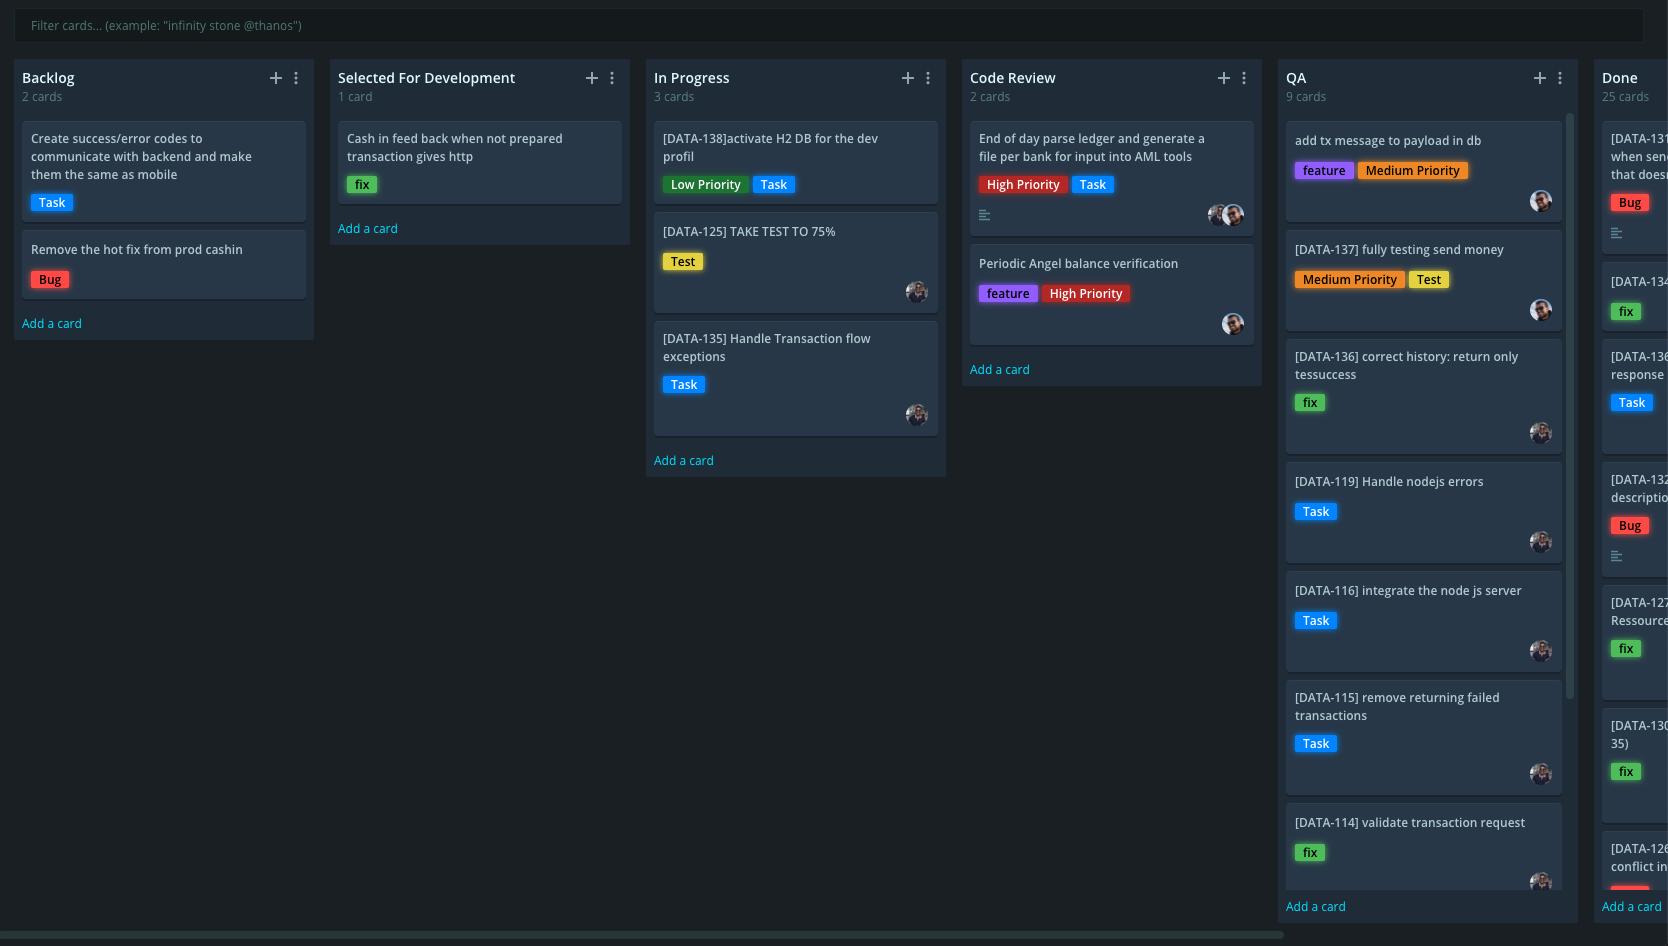
\includegraphics[scale=0.3]{kanban_board.png}
\caption{Kanban Board}
\label{fig:kanban}
\end{figure}
\subsection{Backlog}
All tickets are created in the "Backlog" stage, any work that needs to be done is formed into a ticket.\newline

The ticket needs to have a self-explanatory description to make it simple for the developer to start working on it without the need for further explanation.
\newline

A Tag must be assigned to the ticket as well. Tags may refer to the nature of the work to do (e.g. Bug, Fix, Task), or the scope e.g. Back-end, Front-end, DevOps.
\newline

In the end, the ticket priority must be set following a priority system decided by the development team. The system could rely on numerical values (e.g. 0 having the least priority, 1, 2), or having specific tags (e.g. LOW, MEDIUM, HIGHT, URGENT) which we will be using in our project.
\newline

Tickets can only move from "Backlog" to "Selected For Development".
\subsection{Selected For Development}
In the "Selected For Development" stage developers have access to the tickets. They have to tackle the ticket following the priority system and the tag matching their expertise (back-end, front-end).

Once they choose a ticket they must assign it to their name, move it to the "In Progress" stage and create a git branch with the ticket name and finally start developing.

Tickets could only move from "Selected For Development" to "In Progress".
\subsection{In Progress}
The "In Progress" stage serves as a safety mechanism to avoid having two developers working on the same ticket.

This stage indicates that the tickets are being taken care of and also shows the person developing the ticket.

If the developer finishes his work, he should move the ticket to "Code Review" stage and make a pull request off the branch.


In the case of failure, the ticket should go back to the "Selected For Development" stage.
\subsection{Code Review}
Once a ticket is in the "Code Review" stage, the project manager should open the pull request and check the code committed by the developer.

In the case of approval, the pull request is merged and deployed, the ticket then is moved to "QA".


In the case of disapproval, the project manager leaves comments on the pull request and moves the ticket back to "In progress". The developer then needs to check the code and fix the issue.
\subsection{QA}
In the "QA" stage tickets are tested by fellow developers. The functionality of the ticket should be tested on an environment similar to the production environment. The developer should also push the test to the limit and test all edge cases.

If all developers approve that the code is working fine in every possible scenario, the ticket is moved to "Done". Oherwise, the ticket info should be updated with the issues encountered and the ticket is moved back to the "In Progress" stage.

\subsection{Done}
All tickets should finally be moved to the "Done" stage. This stage groups all the work that is done and keeps track of the progress of the development.


After a fixed time, tickets get archived to gain space in the Kanban board.

\section{Gitflow workflow }
Gitflow Workflow is a Git workflow design that was first published and made popular by Vincent Driessen at nvie. The Gitflow Workflow defines a strict branching model designed around the project release. This provides a robust framework for managing larger projects.

Gitflow is really just an abstract idea of a Git workflow. This means it dictates what kind of branches to set up and how to merge them together.
The figure \ref{fig:git} shows our different branches and our merging strategy.

\begin{figure}[!ht]\centering
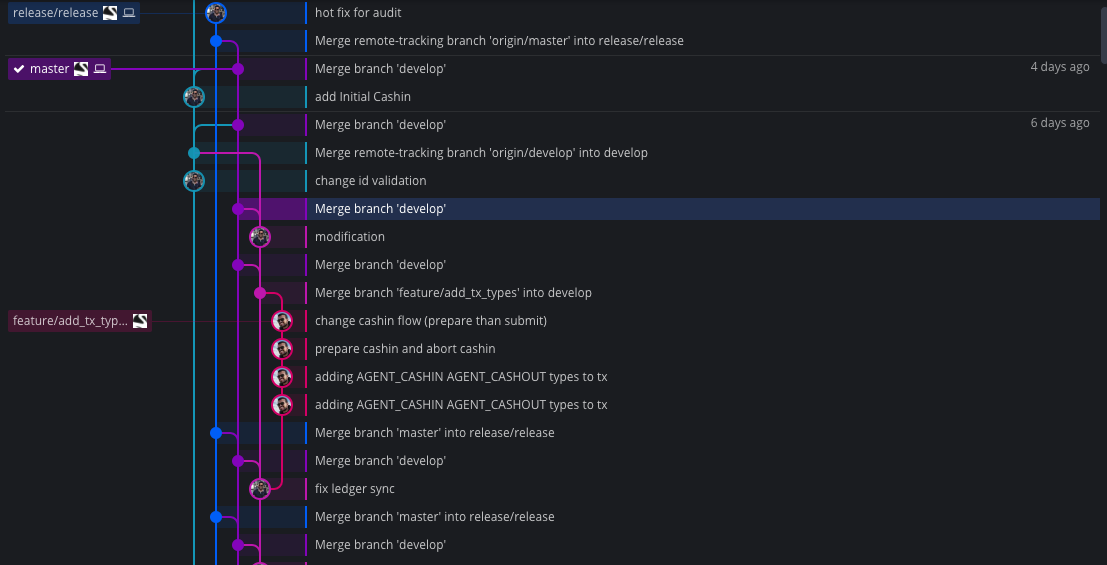
\includegraphics[scale=0.4]{git_workflow.png}
\caption{Git Workflow}
\label{fig:git}
\end{figure}

\subsection{Feature Branch}
The feature branch is created by the developer for every Kanban ticket he tackles. When moving the ticket to the "In Progress" stage, the branch should be created with the same name as the ticket.

All the development specific to the scope of the ticket should be done in the same branch, and in the end, the developer should make a pull request on the Develop Branch.
\subsection{Develop Branch}
The Develop branch presents the edge version of the product, which contains all newly developed features. This branch is the main branch to the internal project team. All newly developed features are tested by developers on this branch, which maps to the "dev environment".

This branch could present a number of bugs because, by nature, it's a testing and validation branch of the latest developed code.

This branch is updated daily.
\subsection{Master Branch}
After tickets validation and bug fixes, the internal team merges a stable version of the product (Develop branch) to the Master branch. This branch maps to the staging environment and serves for testing on the company level.

All company projects depending on our project always use its staging version. The testing and integration with other projects should be verified extensively before merging to the production environment.

\subsection{Release Branch}
This is the production branch, code on this branch has been tested twice in both the dev and staging environments.

The branch is updated according to the release dates. It's the result of merging a stable master branch.

The branch maps to the prod environment and it is the actual branch used by the end user.
\subsection{Hotfix Branch}
As it is impossible to have a bug free software, we should take in consideration bugs popping in the prod environment.

Every bug discovered on the prod environment opens an urgent fix ticket, the ticket branch is based on the release branch and it's merged directly to the release branch after the fix.

This is a measure to quickly fix issues that have effects on the end user.




\section{Test-driven development}
"Test Driven Development" \cite{TDD} is a development technique that requires the writing of tests even before writing the first line of code.

In theory, the method requires the intervention of at least two different people, one who writes the tests, and the other who writes the code. This avoids problems related to subjectivity.

In practice, things are more complicated. Sometimes you develop alone or you write the tests yourself that guarantee the integrity of new functionality in a collaborative project.

The TDD can be divided into 5 distinct steps as shown in the figure  \ref{fig:tdd}:
\begin{enumerate}
	\item  Write a test.
	\item Check that it fails.
	\item Write the code enough for the test to pass.
	\item Check that the test passes.
	\item Optimize the code and check that there is no regression.
\end{enumerate}

\begin{figure}[H]\centering
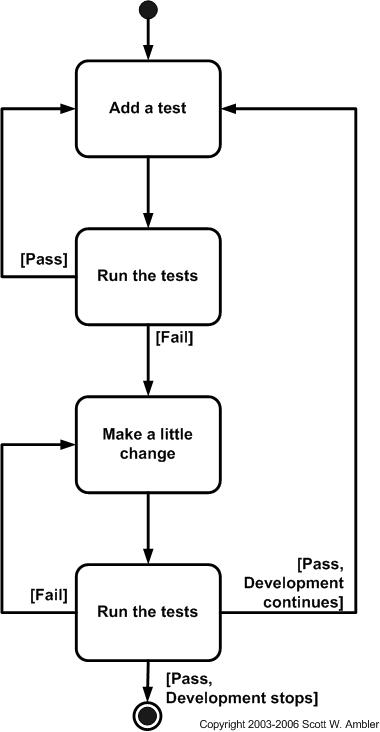
\includegraphics[scale=0.6]{tddSteps.jpg}
\caption{TDD Steps}
\label{fig:tdd}
\end{figure}

In our project, the development of every ticket starts by writing the test. A pull request can only be approved if it contains and passes the new test.

This discipline enables our project to benefits from the DevOps world, as it's important to have a test for the CI-CD process to be defined.


\section{DevOps}
DevOps \cite{devops} is a set of practices that automates the processes between software development and IT teams, in order that they can build, test, and release software faster and more reliably.

In our project, we need to have an autonomous testing and deployment process to maintain our three environments:
\begin{itemize}
	\item \textbf{Dev environment:} Represents the Develop branch and used for internal team testing.
	\item \textbf{Staging environment:} Represents the Master branch and used for a company level testing.
    \item \textbf{Prod environment:} Represents the Release branch and used by the end user.
\end{itemize}

With every branch push, our CI-CD server (Jenkins) triggers an automatic script that consists of a set of predefined steps.

The steps behave slightly different according to the branch name.
Our pipeline is shown in the figure \ref{fig:jenkins}
\begin{figure}[!h]\centering
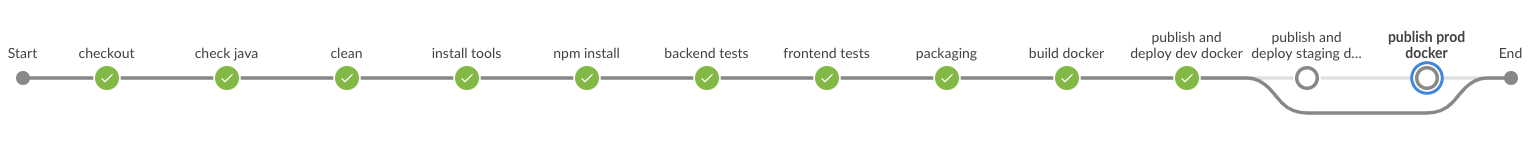
\includegraphics[scale=0.3]{jenkins.png}
\caption{DevOps Pipeline}
\label{fig:jenkins}
\end{figure}
\subsection{Preparation}
The first step of every build is getting the branch code and preparing a clean environment containing all the dependencies required to run our project.
\subsection{Testing}
In this step, all tests are executed for both backend and frontend. A full report is created with the test results.
We can only continue the build if all tests are passed gracefully. Otherwise, the job is terminated.
\subsection{Quality Measurements}
In this step, the code is inspected by the open-source platform SonarQube.

The step performs automatic reviews with static analysis of code to detect bugs, code smells, and security vulnerabilities.
\subsection{Dockerization}
If all testing and quality measures are approved, we proceed to the Dockerization of our project.
\newline

This step creates a standard artifact that can be deployed on any infrastructure without the need for specific configurations for different servers.

If the Docker images are created successfully, it will be tagged latest and pushed to the Docker Hub.

\subsection{Deployment}
In the last step of the build, and according to the branch name the new artifact is deployed to the convenient server (dev, staging, prod).

On every target server, we have a docker swarm cluster to deploy the new version of the product.
The swarm cluster is also configured with the different environment variables as secrets to protect the different credentials (database, cloud services\dots).

\section{General Architecture}
Now that we have defined our development process disciplines and the tools we will be using, we can take the last step before going into the implementation.

In this section, we will discuss the general architecture of the whole project.

In order to integrate Flouci web payment solution, we decided to manage integrations with apps. Every e-commerce website maps to an integration app created on our servers. The app will be linked to the Flouci wallet, and it will hold both public and private keys.
\begin{itemize}
	\item \textbf{Public APP Key:} Used to integrate Flouci form in the e-commerce front-end.
	\item \textbf{Private APP Key:} Used in the e-commerce back-end to verify and accept payments.
\end{itemize}
 The figure \ref{fig:garch} shows the multiple pieces that make it possible to have Flouci as a web payment solution. Arrows show  the interactions between the different pieces. The green key represents the integration app public key and the red key represents the private.

\begin{figure}[H]\centering
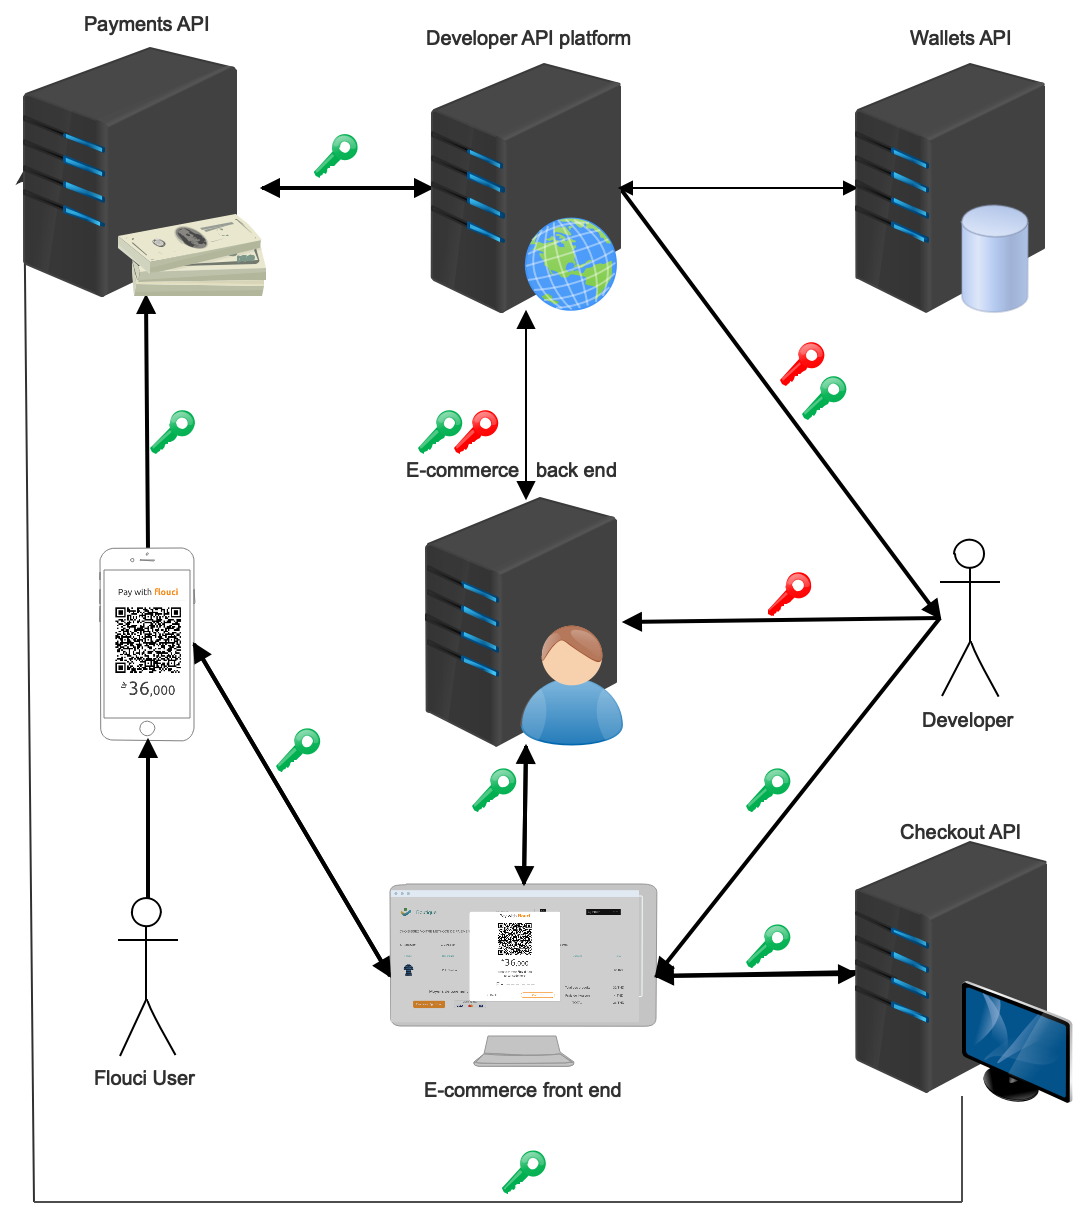
\includegraphics[scale=0.4]{generalarchitecture.png}
\caption{Online Payment General Architecture}
\label{fig:garch}
\end{figure}

\begin{itemize}
	\item \textbf{Developer API platform:} The platform is our central orchestrator, it serves to create integration app's and manage orders.
	\item \textbf{Checkout API:}  Used to integrate Flouci on e-commerce websites.
	\item \textbf{Payments API:}  Used to make payments.
	\item \textbf{Wallets API:}  Used to link wallets to integration apps.
	\item \textbf{E-commerce Front-end:} Contains the Flouci form that generates QR codes linked to specific integration Apps.
	\item \textbf{E-commerce Back-end:} Verify and accept payments.
	\item \textbf{Flouci mobile APP:} Send money through the QR code generated by the front end.
\end{itemize}

\section*{Conclusion}
We went through the Kanban methodology in practice, explaining the different steps of the incremental code writing.

 We also set the rules of the git branching model we will be using in our development process, as well as the test-driven development discipline to follow for every branch.

We tackled our DevOps setup and the different steps of the automation process from code writing to project deployment.


In the end, we studied the general architecture of our project. We also gave a brief description of each component role.

In the next chapter, will start our first sprint entitled "User and App Management". The sprint will contain all steps from design to features implementation.


%==============================================================================
\end{spacing}
